\subsection{Question 4: Disturbance Rescheduling and Strategy Comparison}\label{sec:q4}

\subsubsection{Event Model and State Capture}

The refined margin-compliant Q2(2) schedule of Section~\ref{sec:q22}
($t_{\mathrm{last}}=10.651\,\mathrm{s}$; alert starts $2.388/7.501/10.651\,\mathrm{s}$)
is the operating baseline. At $t=5\,\mathrm{s}$ a disturbance occurs;
the evaluation window is $[0,60]\,\mathrm{s}$. Three primitive events, used alone or in
combination, generate 86 test scenarios:
\begin{itemize}
\item \textbf{(a) New alert.} $T_4=O+R(\cos\theta,\sin\theta)$, $H=50\,\mathrm{m}$
(same polar convention as $T_1$--$T_3$); $\theta$ swept over
$15^\circ{:}30^\circ{:}345^\circ$, $R\in\{30,40,50\}\,\mathrm{m}$ (36 grid points).
\item \textbf{(b) Vehicle failure.} One of V1--V5 exits the field (non-obstructing);
any alert whose joint observation has \emph{not} started and whose assigned pair
contains the failed vehicle is lost under a no-response policy.
\item \textbf{(c) Communication outage.} Orders issued in $[5,t_{rec}]$ cannot reach
the vehicles, which continue on the original plan; new orders take effect upon
recovery, so the decision epoch is $\tau=t_{rec}$.
\end{itemize}
At the decision epoch $\tau$ the dispatcher captures the true state: alerts whose joint
observation already started are \emph{locked} (non-reschedulable; $T_1$ is always
locked since it started at $2.388\,\mathrm{s}<5\,\mathrm{s}$); vehicles are described
by position, current pan/tilt attitude, and free time; reassigned vehicles travel from
their \emph{current} position. A vehicle that is mid-slew toward a committed
observation is captured \emph{at its committed attitude} with that task recorded as a
\emph{commitment}: retaining the identical (alert, station) task inherits the planned
ready time, whereas any retargeting travels and slews from the captured state. No
clairvoyance is allowed: neither P0 nor P1 knows the disturbance before it happens.

\emph{Metrics.} With $N$ alerts to observe in the window (locked + open + new) and $k$
alerts whose joint observation successfully starts, the lexicographic objective is
\begin{equation}\label{eq:q4metric}
\max\ \eta=\frac{k}{N},\qquad\text{then}\quad\min\ t_{\mathrm{last}}
=\max_{\text{alert }a}\{\text{start time of }a\},
\end{equation}
and an alert that never starts within the window forces $t_{\mathrm{last}}=60\,\mathrm{s}$.

The rescheduling model in one block: \emph{given} the captured states at epoch $\tau$
(vehicle positions, gimbal attitudes, free times; locked alerts removed), \emph{choose}
for each open alert two distinct available vehicles and one station of each inside its
observable region---with \emph{no cap} on how many alerts a vehicle may serve (the
problem statement imposes none in the disturbance response; the two-slot restriction of
Section~\ref{sec:q22} is an enumeration convention adopted there, and its cost under
disturbance is quantified below as a control)---and azimuth gap $\ge1^\circ$, \emph{to
optimize} Eq.~\eqref{eq:q4metric} lexicographically---the same
feasible set as Eq.~\eqref{eq:minmax} with the captured states as initial conditions,
and $P_2$ constrained to the rule form stated below.

\subsubsection{Strategies}

\begin{itemize}
\item \textbf{P0 (retain).} Execute the original plan unchanged. Analytic evaluation:
locked alerts count as covered; an open alert paired with the failed vehicle is lost; the
new alert, absent from the plan, stays pending ($t_{\mathrm{last}}=60$).
\item \textbf{P1 (event-triggered re-optimization, cap-free).} At epoch $\tau$, re-solve
the model on the captured states with two complementary \emph{cap-free} searches:
(i) an exhaustive enumeration of (execution order, vehicle pair) structures---at most
3 open alerts and $\binom{5}{2}$ pairs each, $\le6\times10^{3}$ structures, each timed
by an exact event-driven timeline---refined by station-level coordinate descent on the
global objective; and (ii) the Section~\ref{sec:q22} machinery (greedy screening
$\to$ exact simulation $\to$ certified local station search) with the slot cap
removed.  The better plan is deployed; obstacle-aware travel and azimuth gap
$\ge1^\circ$ are enforced throughout, optimizing Eq.~\eqref{eq:q4metric}
lexicographically.
\item \textbf{P2 (rule-based greedy).} An interpretable dispatcher: each round selects the
alert with the earliest achievable completion and assigns the best currently free vehicle
pair by minimum joint readiness, iterating until no assignment improves.
\end{itemize}

To isolate the cost of the two-slot convention, the previous search---enumeration
restricted to at most two task slots per vehicle---is retained as a \emph{control},
denoted $P_{1c}$.

The 86 scenarios (Table~\ref{tab:q4design}) combine the primitives: (a) 36; (b) 5; (c) 5
outage lengths; (a+c) 24 grid points at $t_{rec}\in\{10,30\}$ plus 4 sweep refinements;
(b+c) 5; (a+b) 5 with the \emph{per-vehicle worst-case} alert position; (a+b+c) 2. The
grid quantifies geographic difficulty, the sweeps resolve the time dependence, and the
combination families test whether penalties superpose.\footnote{AI-assistance
annotation (2/3): the scenario batching, state capture and replay-evaluation code for
this subsection was implemented with the help of an AI pair-programming assistant; the
scenario design, the strategy definitions and all result interpretations are the
team's own (see the Declaration in the Appendix and Appendix~B).}

\begin{table}[!htb]\centering
\caption{Scenario design: 86 cases in 7 families ($\tau$ = decision epoch).}
\label{tab:q4design}
\begin{tabular}{llll}
\toprule
Family & Disturbance & $\tau$ & Count \\
\midrule
(a)  & new alert $T_4(\theta,R)$, $H=50$          & 5           & 36 \\
(b)  & single vehicle failure (V1--V5)            & 5           & 5  \\
(c)  & outage only, $t_{rec}\in\{10,15,20,25,30\}$& $t_{rec}$   & 5  \\
(a+c)& new alert + outage                         & $t_{rec}$   & 28 \\
(b+c)& failure + outage ($t_{rec}=10$)            & 10          & 5  \\
(a+b)& new alert at per-vehicle worst $\theta$ + failure & 5    & 5  \\
(a+b+c)& triple                                  & 10          & 2  \\
\bottomrule
\end{tabular}
\end{table}

\subsubsection{Results}

\textbf{(a) New alert (Fig.~\ref{fig:q4agrid}a).} P0 is constant and bad:
$T_4$ stays pending, $\eta=0.75$, $t_{\mathrm{last}}=60$. P1 attains $\eta=1$ in
\emph{all} 36 cells with $t_{\mathrm{last}}\in[15.02,\,17.23]\,\mathrm{s}$---and the
winning plans show that free chaining turns insertion into \emph{re-sequencing}. In
the representative cell $\theta=15^\circ$, $R=40$: V1 is re-aimed $1\,\mathrm{m}$ at
its standby corner to open $T_2$ at $5.35\,\mathrm{s}$ (V4 keeps its committed
station), V2 is re-aimed within its committed station's neighbourhood to give $T_4$
an early southern bearing at $10.54\,\mathrm{s}$ beside V5's northern one (both
near-zero-travel), and the binding chain becomes V1's \emph{second} corner
observation, opening $T_3$ at $15.33\,\mathrm{s}$ while V3's commitment is untouched.
The hardest cell ($\theta=255^\circ$, $R=40$, $17.23\,\mathrm{s}$) binds instead on
V1's $T_3\!\to\!T_4$ chain; the easiest ($\theta=45^\circ$, $R=40$, $15.02\,\mathrm{s}$)
on a northern $T_2$ pair. The cap matters exactly here: restoring the two-slot
convention ($P_{1c}$) is slower in 13 of 36 cells, by up to
$+2.40\,\mathrm{s}$ ($\theta=15^\circ$, $R=40$: $17.73$ vs $15.33$), because a
capped V1 cannot serve the two corner observations; $P_{1c}$'s band is
$[15.02,\,18.10]\,\mathrm{s}$. P2 also reaches $\eta=1$ everywhere but peaks at
$21.16\,\mathrm{s}$ ($\theta=15^\circ$, $R=40$), a greedy trap that chains the wrong
pair first.

\textbf{(b) Vehicle failure (Fig.~\ref{fig:q4agrid}b).} Failing V1--V4 destroys exactly
one open pair ($T_2$'s V1$+$V4 or $T_3$'s V2$+$V3), so P0 drops to $\eta=2/3$; P1
restores $\eta=1$ at $t_{\mathrm{last}}=12.14\,\mathrm{s}$ \emph{identically for all
four}---the re-optimizer routes the disrupted alert through the standby corner and the
freed partner at the single price of $+1.49\,\mathrm{s}$ over the baseline's
$10.651\,\mathrm{s}$. Failing V5 is benign: V5 belongs to no open pair, so P0 already
keeps $(1,\,10.651)$ and re-optimization leaves it unchanged---the refined baseline is
already tight enough that no re-pairing gain exists.

\begin{figure}[!htb]\centering
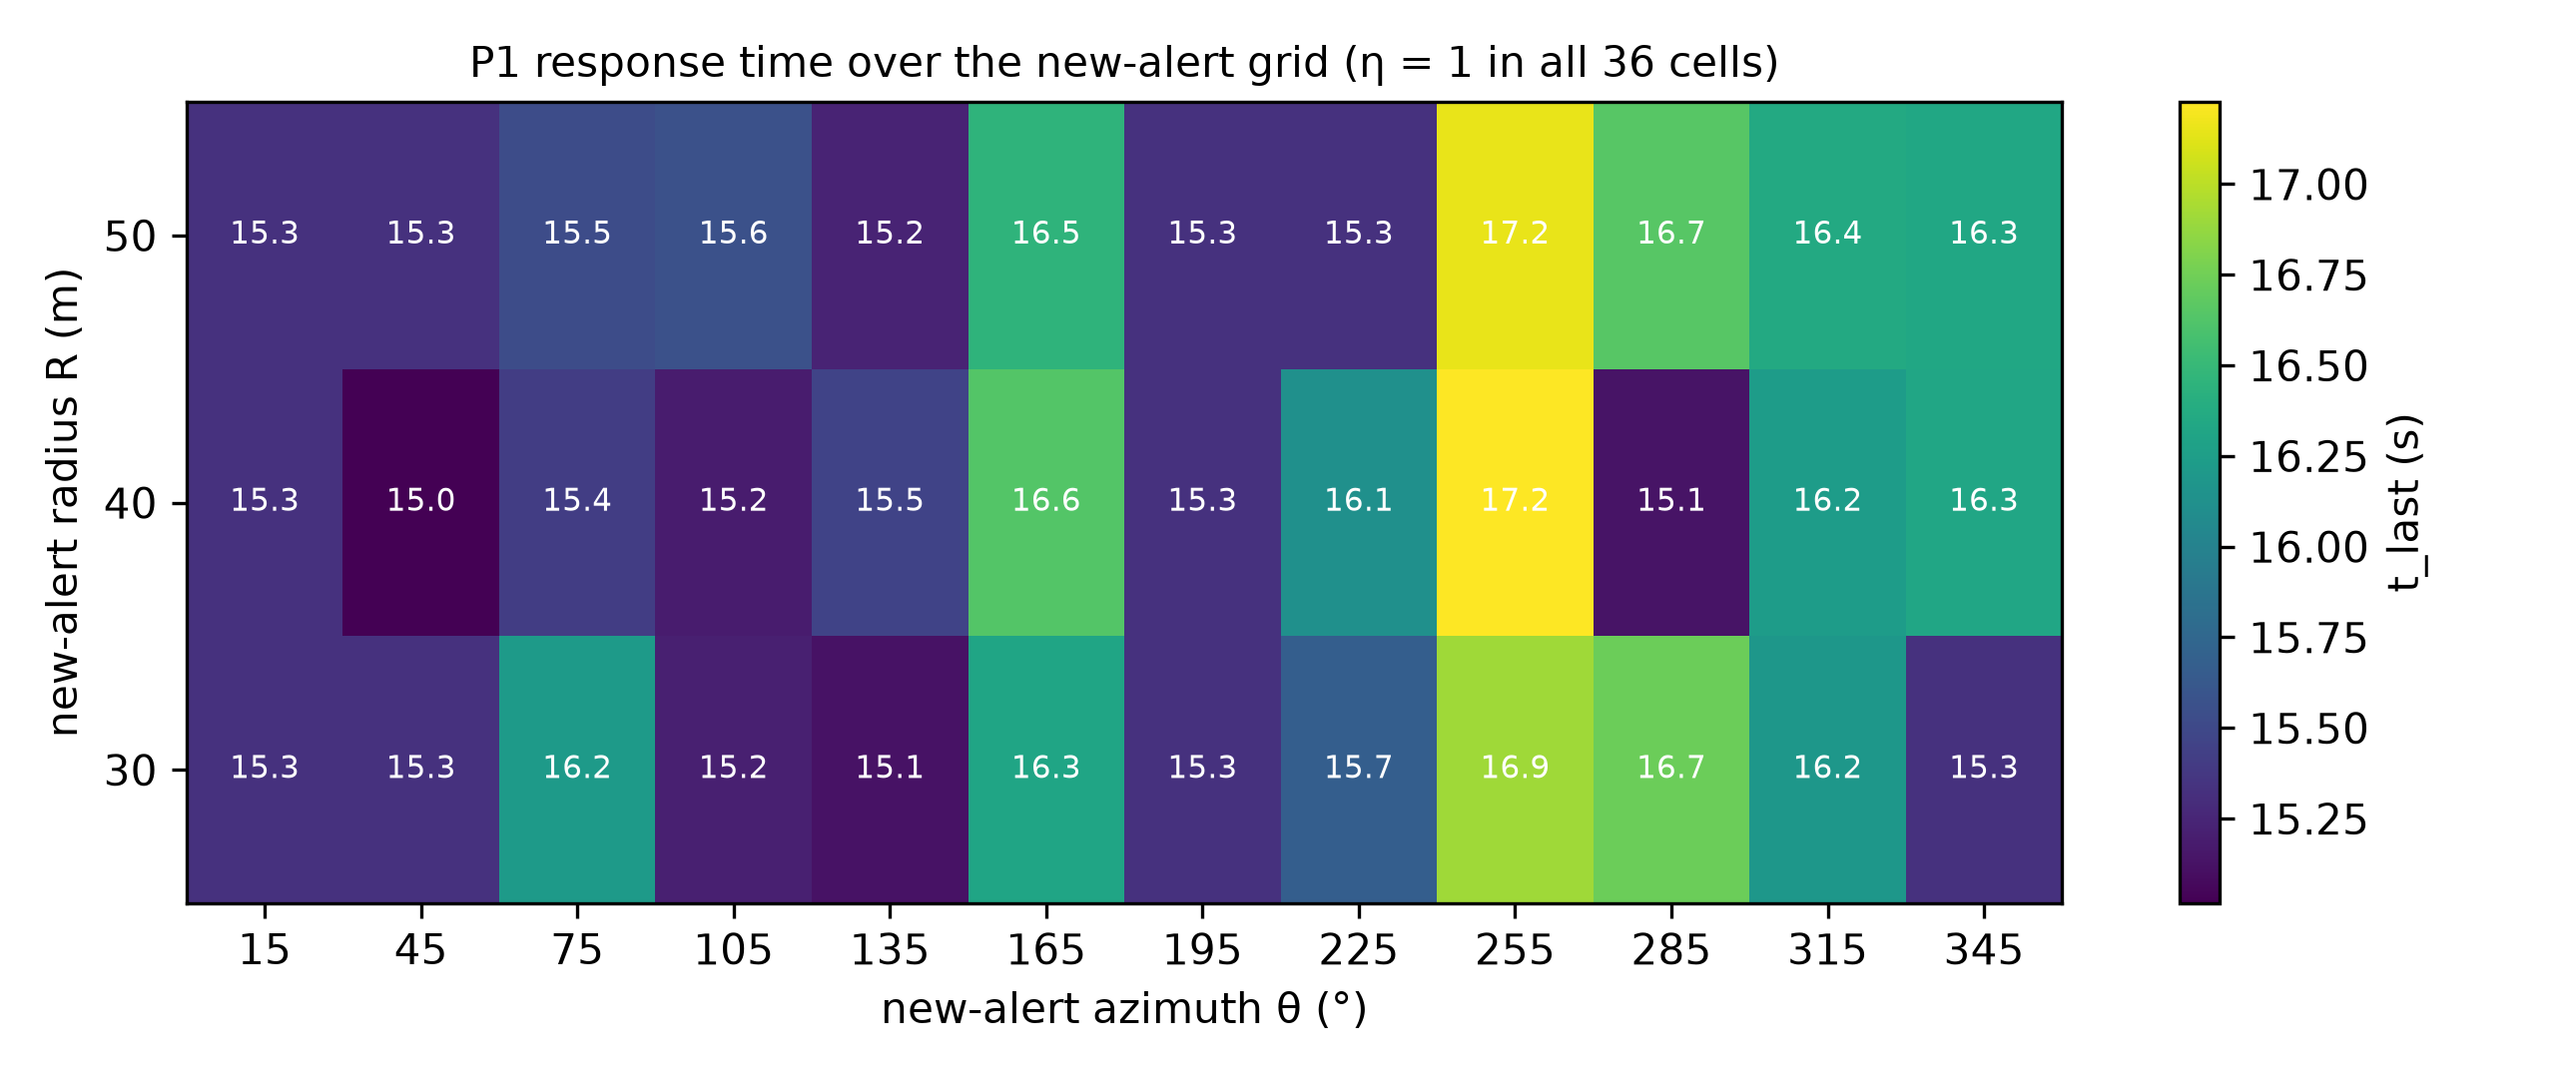
\includegraphics[width=0.42\textwidth]{fig_q4_a_grid.png}\hfill
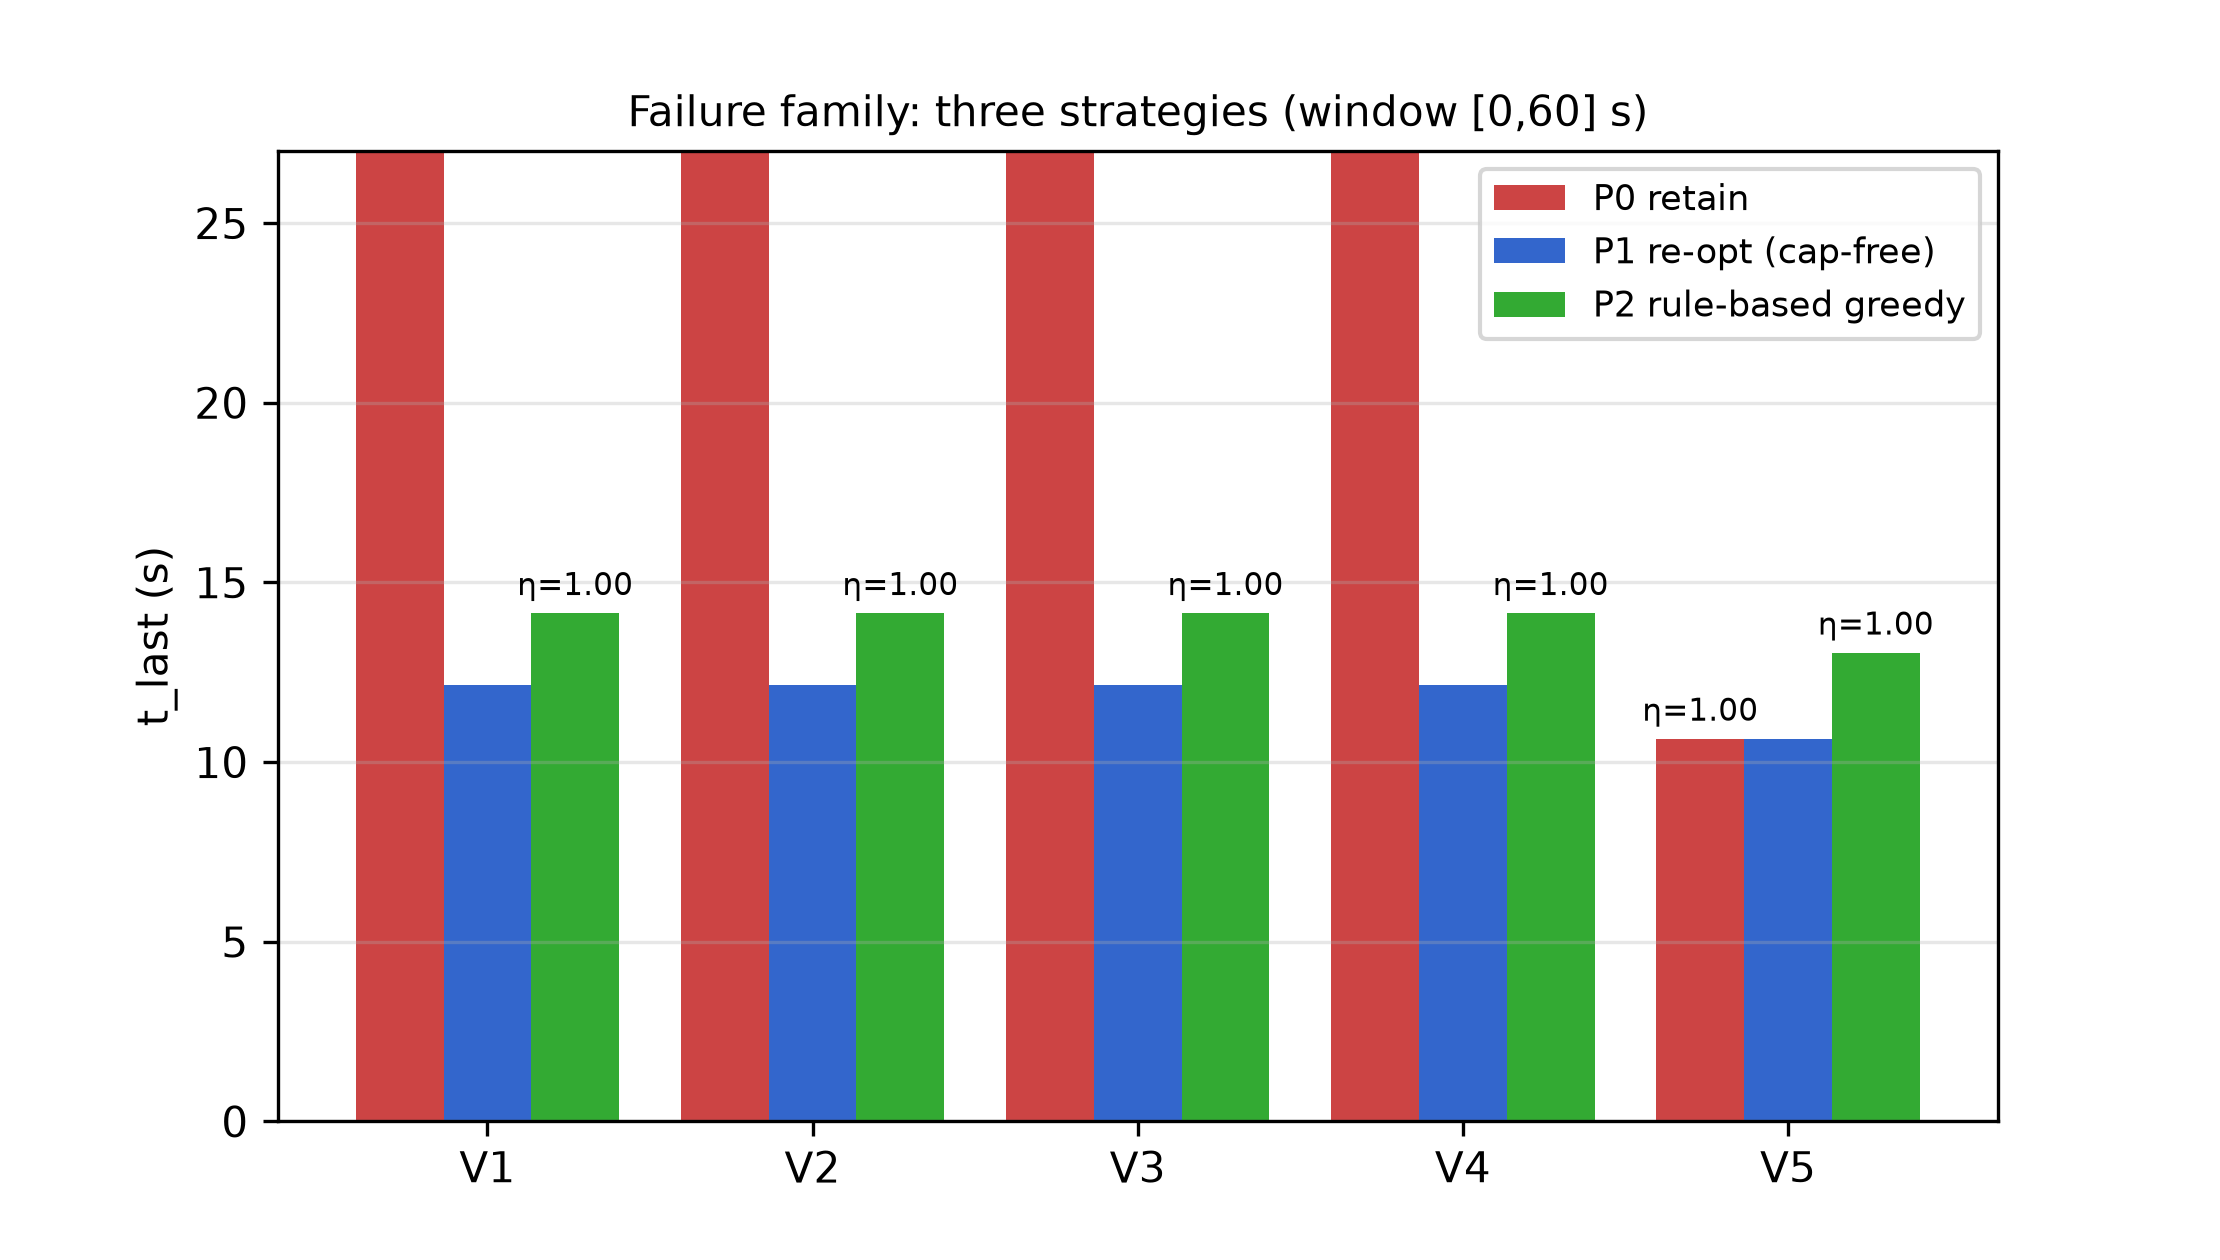
\includegraphics[width=0.42\textwidth]{fig_q4_b_bars.png}
\caption{Family (a) (left): P1 response time $t_{\mathrm{last}}$ over the new-alert grid
(36 cells, $\eta=1$ everywhere; P0 constant at $\eta=0.75$, $t_{\mathrm{last}}=60$).
Family (b) (right): $t_{\mathrm{last}}$ by strategy for each failed vehicle---V1--V4
failures are interchangeable for P1 ($12.14\,\mathrm{s}$); V5 is the only failure the
original plan absorbs by itself.}
\label{fig:q4agrid}
\end{figure}

\textbf{(c) Pure outage: the value boundary.} For $t_{rec}\ge15$, \emph{all four
strategies coincide} at $(\eta,t_{\mathrm{last}})=(1,\,10.651)$: every alert is locked,
leaving nothing to decide. The $10\,\mathrm{s}$ edge is the one live decision---$T_3$
is still open---and the optimal response is a $1^\circ$ re-aim of V3's committed
gimbal inside its neighbourhood ($10.34\,\mathrm{s}$, $-0.31\,\mathrm{s}$, identical
for P1 and $P_{1c}$). The rule-based P2, blind to commitments, re-pairs $T_3$ instead
and \emph{loses} $2.6\,\mathrm{s}$ against doing nothing ($13.22\,\mathrm{s}$): without
the commitment mechanism, rescheduling can be worse than retaining. This family
delimits \emph{when} rescheduling is worthless---a plan should not be disrupted while
it still works.

\textbf{(a+c) Outage + new alert (Fig.~\ref{fig:q4trec}, left).} Once a decision must
actually be made, delay becomes expensive in steps, not smoothly: with $T_4$ at
$R=40\,\mathrm{m}$, P1 holds a $17.52\,\mathrm{s}$ plateau for $\tau\le10$ (the joint
re-timing of $\{T_3,T_4\}$ is already optimal), rises to $18.88\,\mathrm{s}$ once $T_3$
locks mid-observation ($\tau\in[12.5,15]$---the joint option vanishes), and then
degrades at $\approx0.85\,\mathrm{s}$ per second of outage up to
$31.62$--$33.46\,\mathrm{s}$ at $\tau=30$. The cap costs $+1.25\,\mathrm{s}$ at the
first plateau ($P_{1c}$: $18.77$ vs $17.52$ at $\tau=7.5$) where the corner chain is
forbidden. Outage hurts roughly one-to-one while it lasts, because it freezes both the
information channel and the repositioning clock, with plateaus while the fleet is
committed.

\begin{figure}[!htb]\centering
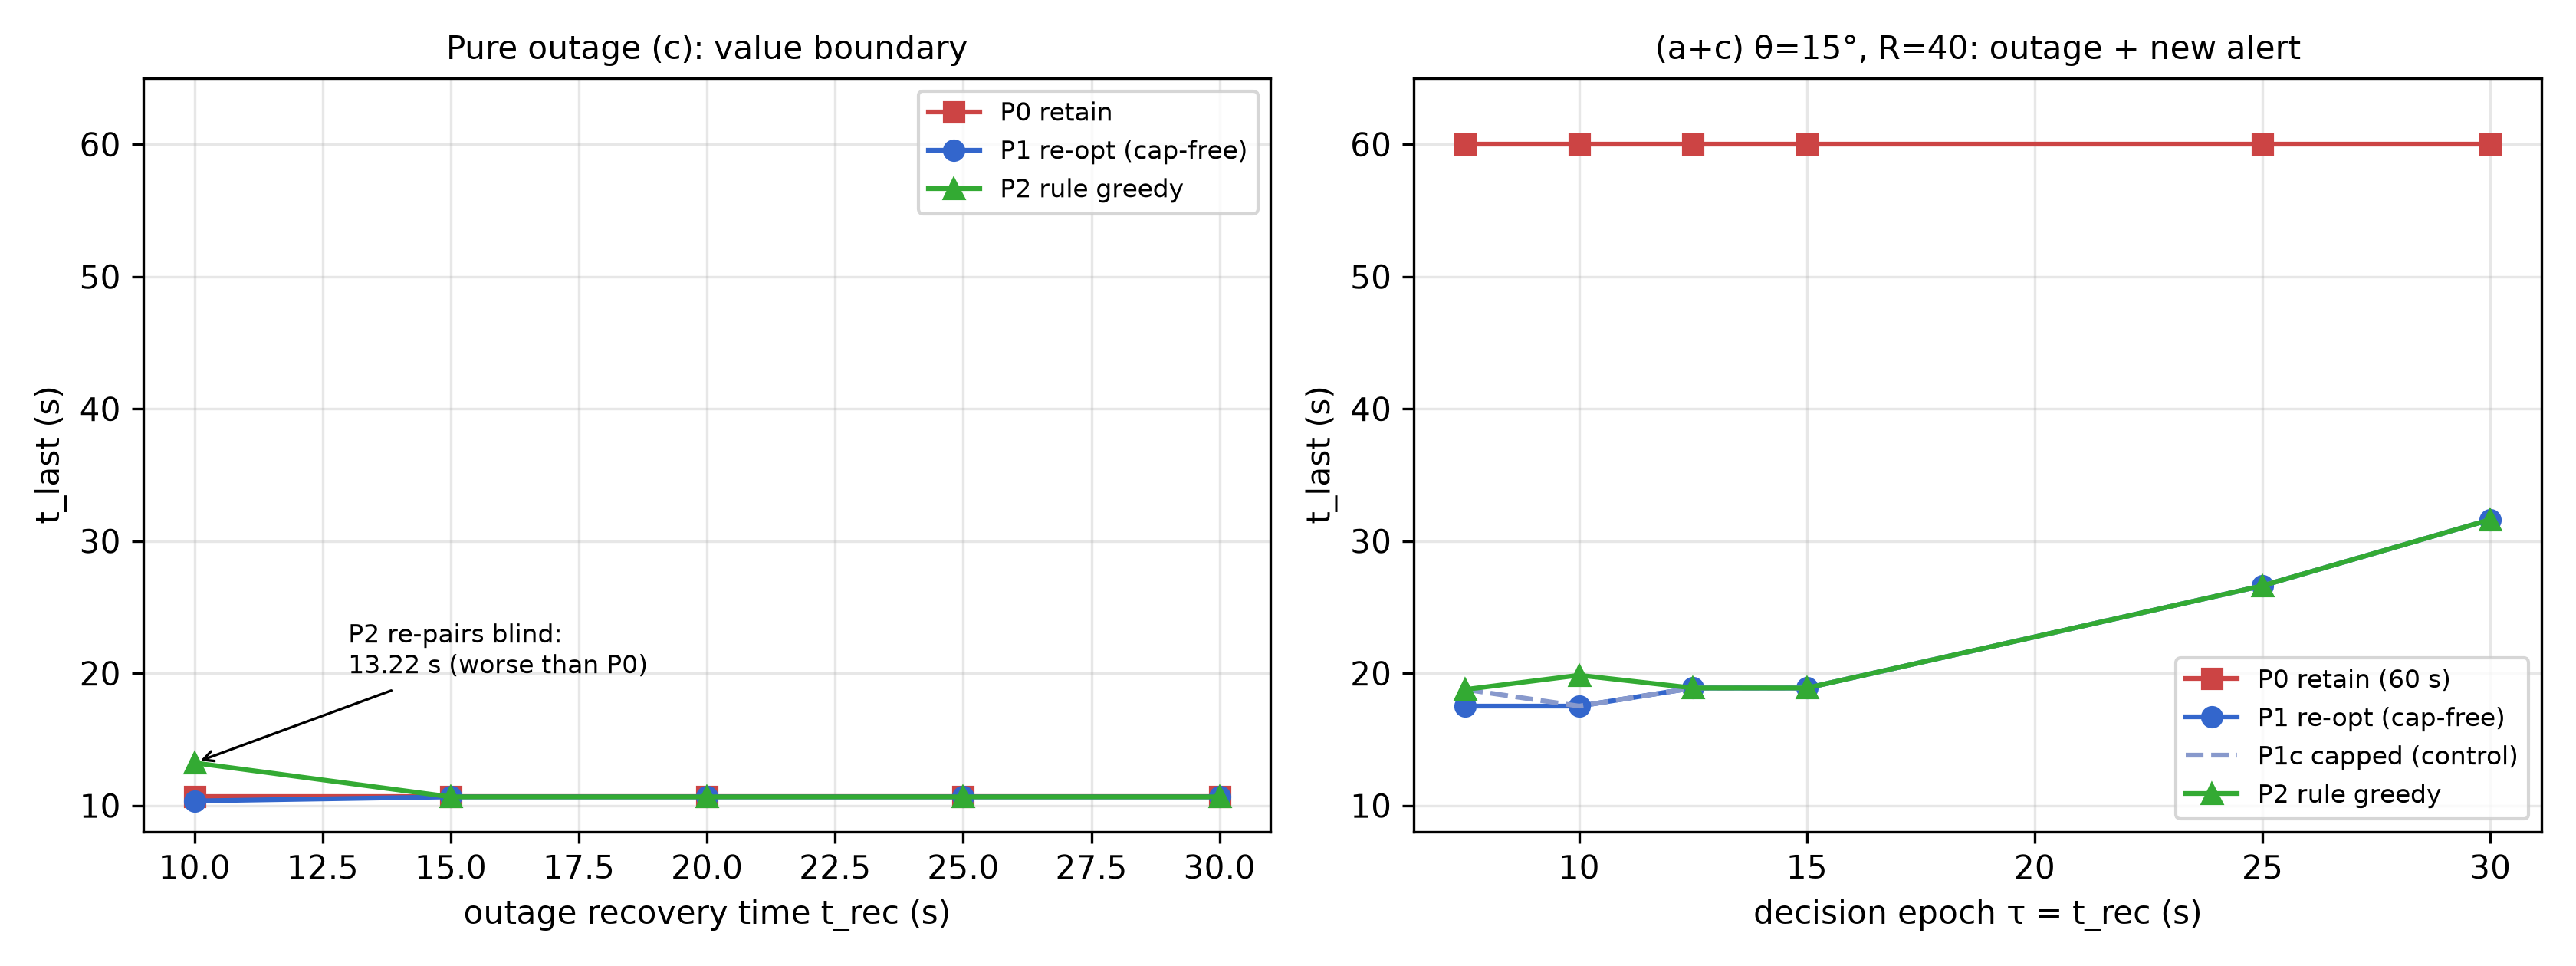
\includegraphics[width=0.42\textwidth]{fig_q4_trec.png}\hfill
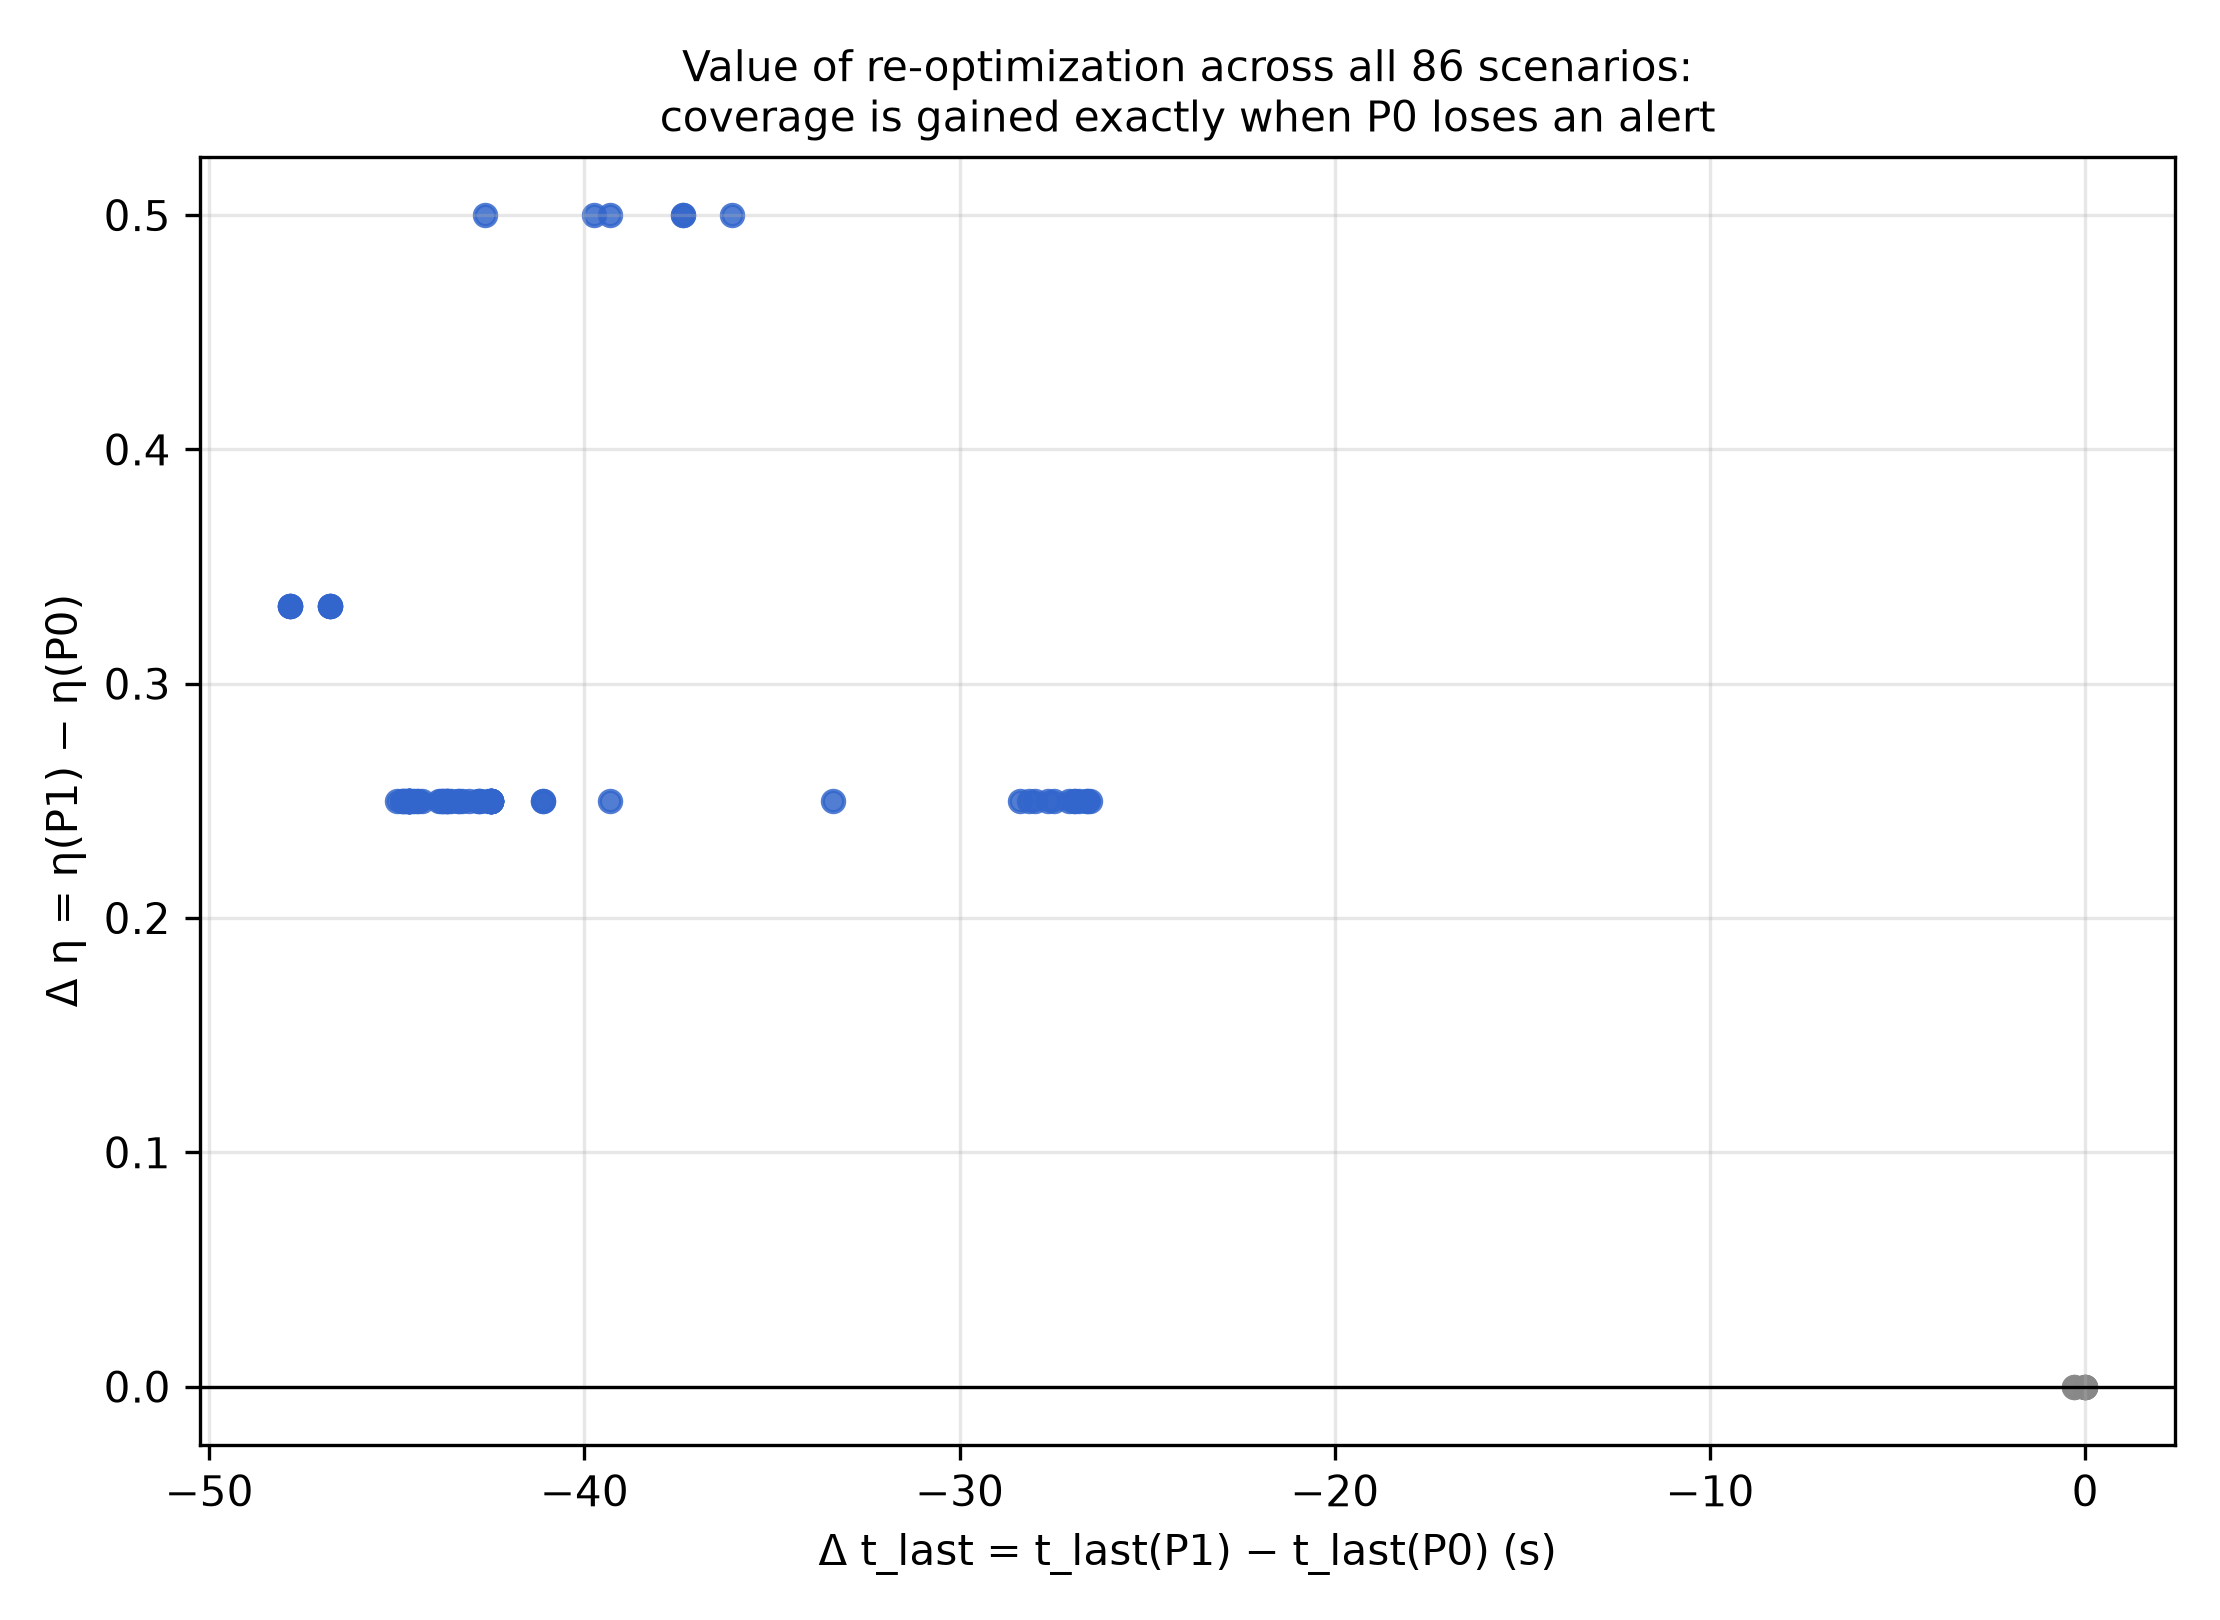
\includegraphics[width=0.36\textwidth]{fig_q4_value.png}
\caption{Left: pure outage (c)---all strategies coincide at $10.651\,\mathrm{s}$ for
$t_{rec}\ge15$ (zero gain), but P2's commitment-blind re-pairing \emph{loses}
$2.6\,\mathrm{s}$ at the $10\,\mathrm{s}$ edge---and (a+c) at $\theta=15^\circ$,
$R=40$ (P0 at $60\,\mathrm{s}$ throughout; P1 plateaus while the fleet is committed,
then degrades at $\approx0.85\,\mathrm{s}$ per second of outage). Right: value of
re-optimization across all 86 scenarios, $\Delta\eta=\eta_{P1}-\eta_{P0}$ versus
$\Delta t_{\mathrm{last}}$: every scenario gains coverage exactly when P0 drops below
$\eta=1$.}
\label{fig:q4trec}
\end{figure}

\textbf{(b+c) Failure + outage.} At $\tau=10$: every V1--V4 failure costs
$13.22\,\mathrm{s}$---uniformly, $+1.08\,\mathrm{s}$ over family (b)---and the
benign V5 case still collects the $10.34\,\mathrm{s}$ re-aim gain; the extra
$5\,\mathrm{s}$ of silence is again roughly one-to-one.

\textbf{(a+b) New alert + failure, worst case.} The per-vehicle hardest alert positions
are $\theta=225^\circ$ (V1, V2, V3, V5) and $\theta=135^\circ$ (V4) at $R=40\,\mathrm{m}$.
P0 collapses to $\eta=0.5$ (V5-failure: $0.75$); P1 restores $\eta=1$ with
$t_{\mathrm{last}}\in[17.34,\,23.94]\,\mathrm{s}$---a penalty of $+1.2$ to
$+7.8\,\mathrm{s}$ over the corresponding failure-free cells, i.e.\ the two
disturbances superpose approximately additively rather than multiplicatively. The
V3-failure cell is the mildest ($17.34\,\mathrm{s}$): V2 keeps its $T_3$ commitment and
the standby corner chain covers $T_4$ early. The most instructive case is V5-failure
plus new alert: P0 loses $T_4$ only ($\eta=0.75$), P1 covers all four alerts at
$20.69\,\mathrm{s}$.

\textbf{(a+b+c) Triple.} $V2$-failure and $V3$-failure both resolve at
$22.63\,\mathrm{s}$ ($\tau=10$, $\theta=225^\circ$, $R=40$)---still $\eta=1$.

\textbf{P1 versus $P_{1c}$ and P2.} Across all 86 scenarios the cap-free P1 is faster
than the slot-capped control in 16 (up to $2.40\,\mathrm{s}$, mean $0.18\,\mathrm{s}$),
ties it in 67, and concedes $\le1.63\,\mathrm{s}$ in 3 cells (search-budget
truncation, not structure: both searches are heuristics inside the same
cap-free feasible set). P2 attains $\eta=1$ in all 86 scenarios---the problem is
forgiving enough that a greedy rule never loses an alert---but its $t_{\mathrm{last}}$
deficit reaches $6.07\,\mathrm{s}$ ($(a+b)$, V3-failure: $23.41$ vs $17.34$), is
systematic in failure and new-alert families, and at the outage edge it is the only
strategy \emph{slower than doing nothing}. P1 buys speed with two cap-free searches
that cost milliseconds each; P2 buys explainability at a documented price. Both
dominate P0 everywhere except family (c).

\subsubsection{Validation}

Every P1/P2 plan is evaluated by replaying the event-driven simulator from the captured
states (the same simulator that produced the Q2(2) timeline), so reported start times
are simulation outputs, not analytic estimates; all clearance, azimuth-gap
and attitude-continuation constraints are re-checked inside the replay. Family (b)'s
identity across V1--V4 failures was verified to arise from equal-cost substitutions.

\emph{Cross-study robustness (L3).} A fully independent re-study of the same question
was conducted with the conservative enumerated baseline ($11.046\,\mathrm{s}$), a
45-scenario set, and a coordinate-descent rescheduler; the main 86-scenario study of
Table~\ref{tab:q4design} freezes the refined $10.651\,\mathrm{s}$ schedule instead
(the second study uses a coarser new-alert grid and a different set of combinations).
The second study reproduces every qualitative boundary reported here: full
$\eta=1$ recovery under event-triggered re-optimization, the pure-outage value
boundary (zero beyond $15\,\mathrm{s}$; a convention-level $\le0.31\,\mathrm{s}$ gain
at the $10\,\mathrm{s}$ edge from re-aiming a committed gimbal), the benign
V5-failure case, and approximately additive combination penalties.
Q3's reliability limit applies to cumulative
travel at a $40\,\mathrm{m}$ target range; Q4 does not test it at each observation.
